We have implemented a full Bayesian GP modeling approach with
Pyro. We have applied our implementation to the dataset $\mathcal{D}$ described in the assignment text.
We use NUTS, with a Gaussian RBF kernel, to sample from the posterior $p(\theta | \mathcal{D})$. The priors used for the kernel parameters $\sigma^2_l$ and $\sigma^2_s$ are the ones given in the assignment text.
For hyperparameters, we use $W = 100$ warmup steps and $C = 4$ chains.
In \cref{fig:gp:analysis} we show the ESS and r\_hat values computed for our trained model. We achieve ESS values of above 400, which indicates that our model approximates the posterior distributions of the actual parameters well. Furthermore, we have r\_hat values of 1.01 for both parameters, indicating that the sampling has converged.
\begin{figure}[H]
\begin{tabular}{l l l}
$\sigma^2_l$ & & \\ \midrule
& ESS bulk & 412.0 \\
& ESS tail & 725.0 \\
& r\_hat & 1.01\\ 
$\sigma^2_p$ & & \\\midrule
& ESS bulk & 534.0 \\
& ESS tail & 614.0 \\
& r\_hat & 1.01\\
\end{tabular}
\caption{Effective sample size (ESS) and r\_hat values calculated with Arviz}
\end{figure}
\begin{figure}[H]
    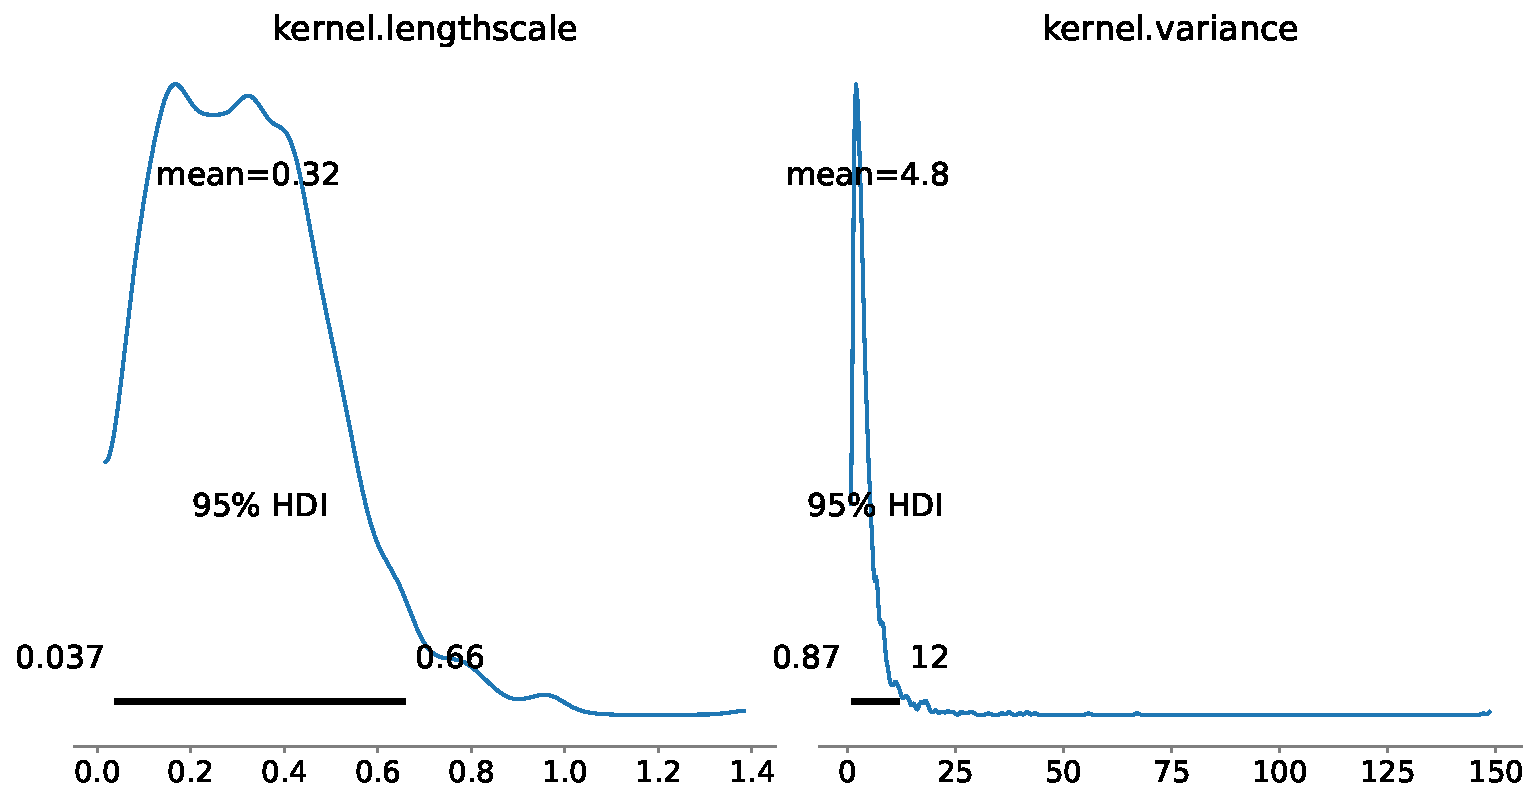
\includegraphics[width=0.49\textwidth]{figures/gp/sample_analysis.pdf}
    \caption{Plot showing the posterior densities of the RBF kernel's learned parameters}
    \label{fig:gp:sample_analysis}
\end{figure}
In \cref{fig:gp:loglog} we show 500 samples from $p(\theta|\mathcal{D})$ from each chain, and in \cref{fig:gp:plot1} we show $p(f^*|x^*, \mathcal{D})$ along with its confidence interval and mean.
\begin{figure}[H]
    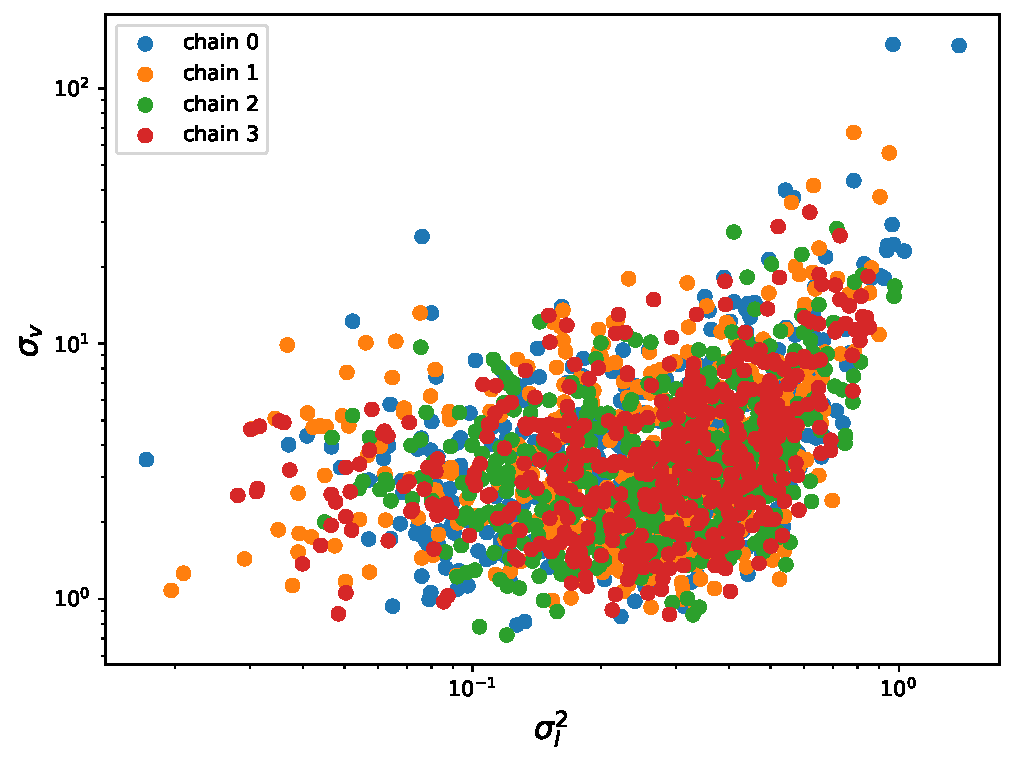
\includegraphics[width=0.49\textwidth]{figures/gp/loglogscale.pdf}
    \caption{Scatter plot on log-log-scale of $N = 500$ samples from $p(\theta | \mathcal{D})$ from 4 chains}
    \label{fig:gp:analysis}
\end{figure}
\begin{figure}[H]
    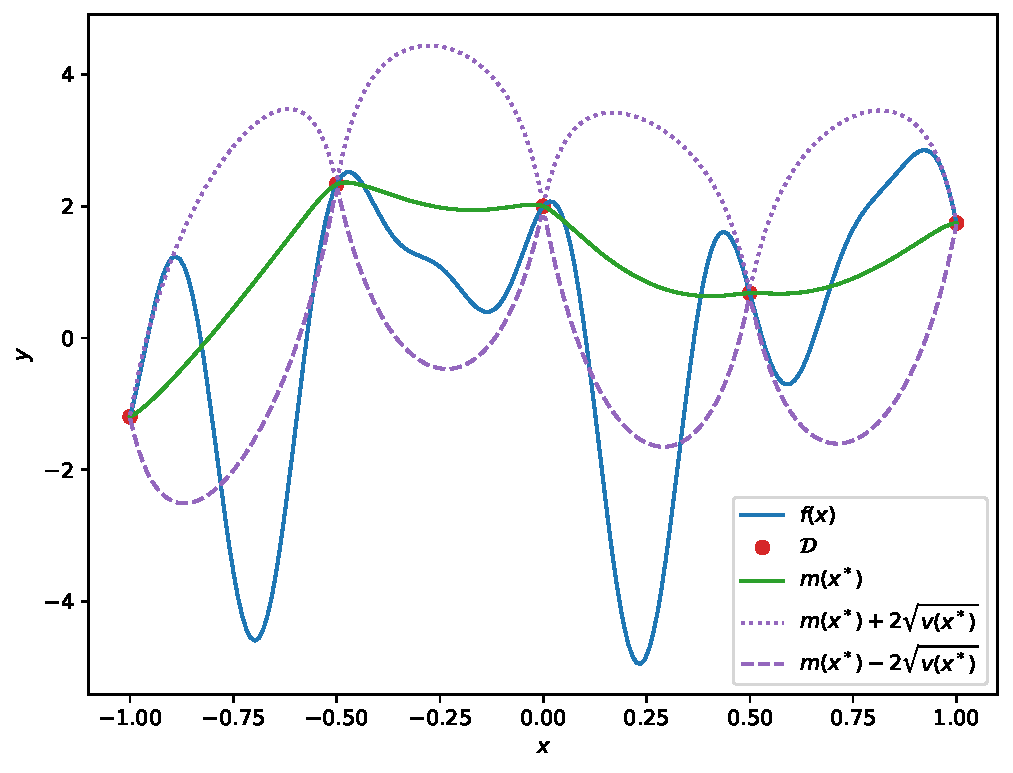
\includegraphics[width=0.49\textwidth]{figures/gp/plot.pdf}
    \caption{Plot of $p(f^*|x^*,\mathcal{D})$ along with its mean and confidence interval}
\end{figure}